\documentclass[10pt]{ctexbeamer}

% \usetheme[logo=UCAS, sublogo=AMSS]{ucas}
\usetheme{ucas}
% logo 的选项: CAS, UCAS
% sublogo 的选项: AMSS, AMSS2018, UCAS

% 引入参考文献列表的 .bib 文件, 使用 GB/T 7714-2015 的文献著录规则.
\usepackage[backend=biber, style=gb7714-2015]{biblatex}
\usepackage[all]{xy}
\usepackage{tikz-cd,amsfonts}
\usepackage{tikz}
\usetikzlibrary{positioning, shapes.geometric}
\usetikzlibrary{shapes.geometric, arrows,chains}
\addbibresource{ref.bib}

\AtBeginSubsection[]{
  \begin{frame}{目录}
    \tableofcontents[currentsection,currentsubsection]
  \end{frame}
} 

\title[title]{叶层化对的Sarkisov纲领}
\author[Yanze Wang]{\href{mailto:wyz2016zxc@outlook.com}{王延泽}}
\institute[AMSS, CAS]{中国科学院数学与系统科学研究院}
\date{2024年5月13日, 思源楼813}
\subject{展示主题}
\keywords{极小模型纲领,Sarkisov纲领,叶层化对}

\begin{document}

\begin{frame}[plain]
  \maketitle
\end{frame}

\begin{frame}[t]
  \frametitle{目录}
  \tableofcontents
\end{frame}

\section{绪论}\label{sec:1}
\subsection{问题背景}\label{subsec:1-1}
\begin{frame}[shrink]
  \frametitle{双有理代数几何和极小模型纲领}
  双有理代数几何的目标之一是按双有理等价类分类代数簇,并选取恰当的代表元。

  \pause
  极小模型纲领 (Minimal model program)是构造代表元的一种方法,并且猜想每一个代数簇都双有理等价于一个极小模型 或一个森纤维空间。
  \begin{itemize}
    \pause
    \item 如果代数簇对$(X,B)$的对数典范除子$(K_{X}+B)$是数值有效 (nef)的,那么称之为\textbf{极小模型(minimal model)};
    
    \pause
    \item 如果存在压缩态射$f:(X,B)\to S$使得$\rho(X/S)=1$且$-(K_{X}+B)$相对于$S$ 丰沛 (ample),则称之为\textbf{森纤维空间 (Mori fibre space)};
  \end{itemize}
% \pause
\end{frame}

\begin{frame}[shrink]
  \frametitle{压缩态射和翻转}
对于klt点的$\mathbb{Q}$-分解代数簇对$(X,B)$,如果$(K_{X}+B)$不是数值有效(nef)的,那么存在压缩态射$f:X\to Z$,分为三种情况:
\begin{enumerate}
    \pause
  \item $f$是双有理态射,$\operatorname{Exc}\,f=E$是素除子,此时称为除子压缩态射 (divisorial contraction morphism);
    \pause
  \item $f$是双有理态射,$\operatorname{codim }(\operatorname{Exc}\,f) \geqslant 2$,则称为小双有理态射 (small birational morphism);
    \pause
  \item $\dim Z < \dim X, \operatorname{Exc}\,f=X$,此时称$(X,B)\to Z$为森纤维空间 (关于$ (K_{X}+B) $的森纤维空间),压缩态射$f$称为森纤维空间压缩态射。
\end{enumerate}
    \pause
对于小双有理态射$f$ ,可以定义翻转 (flip)$f^{+}$ :
    \[ \xymatrix{
        X\ar[rd]_{f} \ar@{.>}[rr] & & X_{1}\ar[ld]^{f^{+}} \\
      & Z & } \]
      其中$B_{1}$为$B$ 在$X_{1}$上的严格双有理变换,$(K_{X_{1}}+B_{1})$相对于$Z$丰沛,且$X \dashrightarrow X_{1}$是余维数$1$同构。
\end{frame}

\begin{frame}[shrink]
  \frametitle{极小模型纲领}
  \pause
对于$(X,B)=(X_{0},B_{0})$,且$(K_{X}+B)$不是数值有效的,对于压缩态射$f_{1}:X\to Z$,
\begin{enumerate}
    \pause
  \item 如果是除子压缩,那么令$X_{1}=Z,B_{1}=f_{1*}B$。在$(X_{1},B_{1})$上重复此过程;
    \pause
  \item 如果是小双有理态射,那么令$f^{+}_{1}:(X_{1},B_{1})\to Z$为$f_{1}$的翻转,在$(X_{1},B_{1})$上重复此过程;
\end{enumerate}

 \begin{itemize}
    \pause
   \item 如果持续做前两种操作,并最终在$(X_{i},B_{i})$上$K_{X_{i}}+B_{i}$是数值有效除子,那么MMP在此终结,且$(X_{i},B_{i})$是极小模型;
    \pause
   \item 如果出现森纤维空间压缩态射$(X_{i},B_{i})\to Z$停止,那么MMP终结于这个森纤维空间。
 \end{itemize} 
\end{frame}

\begin{frame}[shrink]
  \frametitle{极小模型纲领}
\begin{center}
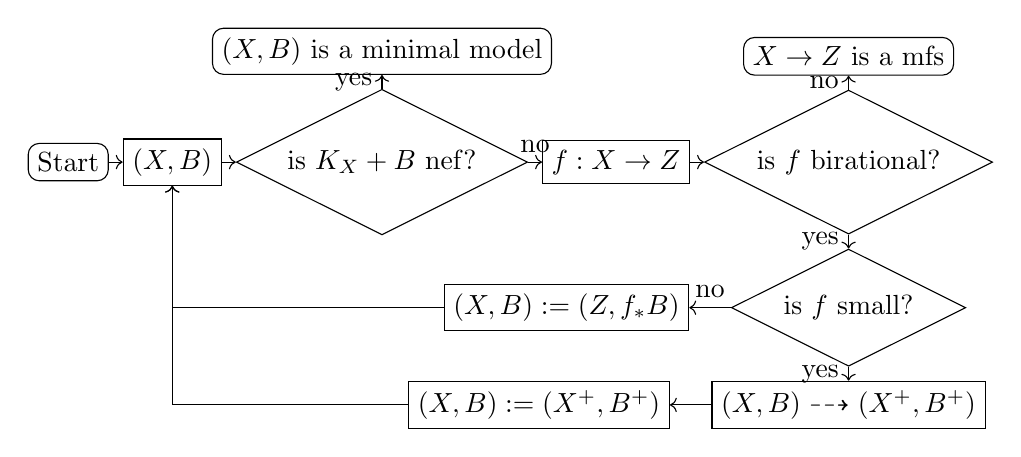
\begin{tikzpicture}[node distance=5pt]
  \node[draw, rounded corners]                        (start)   {Start};
  \node[draw, right=of start]                         (begin)  {$(X,B)$};
  \node[draw, diamond, aspect=2, right=of begin]     (nef)  {is $K_{X}+B$ nef?};
  \node[draw, rounded corners, above=of nef]                   (mm)  {$(X,B) $ is a minimal model};
  \node[draw, right=of nef]                   (cont)  { $f:X\to Z$};
  \node[draw, diamond, aspect=2, right=of cont]     (bir)  {is $f$  birational?};
  \node[draw, rounded corners, above=of bir]                   (mfs)  {$X\to Z $ is a mfs};
  \node[draw, diamond, aspect=2, below=of bir]     (small)  {is $f$ small?};
  \node[draw, below=of small]                         (flip)  {$(X,B) \dashrightarrow (X^{+},B^{+})$ };
  \node[draw, left=15pt of small]                   (div)  {$(X,B):=(Z,f_{*}B)$};
  \node[draw, left=15pt of flip]                         (repflip)  {$(X,B):=(X^{+},B^{+})$};
  
  \draw[->] (start)  -- (begin);
  \draw[->] (begin) -- (nef);
  \draw[->] (nef) -- node[above]  {no} (cont);
  \draw[->] (nef) -- node[left]  {yes} (mm);
  \draw[->] (cont) -- (bir);
  \draw[->] (bir) -- node[left]  {no} (mfs);
  \draw[->] (bir) -- node[left]  {yes} (small);
  \draw[->] (small) -- node[left]  {yes} (flip);
  \draw[->] (small) -- node[above]  {no} (div);
  \draw[->] (div) -- (begin|-div) -> (begin);
  \draw[->] (flip) -- (repflip);
  \draw[->] (repflip) -- (begin|-repflip) -> (begin);
\end{tikzpicture}
\end{center}
\end{frame}

\begin{frame}[shrink]
  \frametitle{极小模型纲领}
  \framesubtitle{MMP-相关}

  上述过程称为$(K_{X}+B)$-MMP,其中出现的代数簇对$(X_{i},B_{i})$被称为MMP的结果,将MMP停止处的代数簇对称为MMP的输出 (极小模型或森纤维空间)。如果考虑相对代数簇对,即考虑基底$U$ 和压缩态射$\pi:X\to U$,也有相应的相对于$U$ 的MMP。

    \pause
  MMP过程得到的代表元有时并不唯一,不同的代表元被称为\alert{MMP-相关}。

    \pause
  \begin{block}{}
对同一个$(X,B)$,虽然代表元不唯一,但一定是相同的类型的代表元。如果$(K_{X}+B)$是伪有效的(pseudoeffective),则代表元是极小模型;否则代表元是森纤维空间。
\end{block}{}
    \pause
\begin{block}{问题}
自然的问题就是不同代表元之间的关系。
\end{block}
\end{frame}




\begin{frame}[shrink]
  \frametitle{连接代表元}
当代表元是不同的极小模型时,有下列定理:
% \pause
    \pause
\begin{theorem}[Kawamata](\citeauthor[Theorem 1]{flopmin})
  令$(W,B_{W})$为一个终端奇点的$\mathbb{Q}$-分解代数簇对,且 $(X,B_{X}), (Y,B_{Y})$是它的两个极小模型。那么双有理映射$X \dashrightarrow Y$可以分解为一系列$(K_{X}+B_{X})$-平转 (也称为复络, flop)的复合。
\end{theorem}
    \pause
当代表元是不同的森纤维空间时,是本论文的主要研究问题:
    \pause
  \begin{theorem}[Sarkisov, Corti, Hacon, Bruno, Matsuki](\citeauthor[Theorem 1.1]{haconSarkisovProgram2012})\label{main}
  令 $ f:(X, B)\to S$ 和 $f':(X', B')\to S' $ 为两个 MMP-相关的klt奇点的$ \mathbb{Q} $-分解森纤维空间,则有双有理映射 $\Phi:(X,B)\dashrightarrow (X',B')$ 可以分解为Sarkisov连接映射的复合,即
  \[ \Phi=\Psi_{n}\circ \cdots \circ \Psi_{1} \]
  其中$\Psi_{i}:X_{i}\dashrightarrow X_{i+1} $ 是四种Sarkisov连接之一。
  \end{theorem}
\end{frame}

\begin{frame}[shrink]
  \frametitle{Sarkisov纲领}
  \framesubtitle{Sarkisov连接}
  Sarkisov连接如下所示:
  \begin{center}
  \textbf{第一型:}$\xymatrix{
      Z\ar[d]_{p}\ar@{.>}[r]&X_{1}\ar[d]^{f_1}\\
      X\ar[d]_{f}&S_1\ar[dl]^{t}\\
  S &}$
  \textbf{第二型:}$\xymatrix{
      Z\ar[d]_{p}\ar@{.>}[r]&X_{1}\ar[d]^{f_1}\\
      X\ar[d]_{f}&S_1\ar[dl]^{t}\\
  S &}$
  \end{center}
  \begin{center}
    \textbf{第三型:}$\xymatrix{
        Z\ar[d]_{p}\ar@{.>}[r]&Z'\ar[d]^{q}\\
        X\ar[d]_{f}&X_1\ar[d]^{f_1}\\
    S\ar[r]^{\sim}&S_1}$
  \textbf{第四型:}$\xymatrix{
      X\ar@{.>}[r]\ar[d]_{f}& Z\ar[d]^q \\
      S\ar[rd]_{s}         & X_{1}\ar[d]^{f_{1}}\\
      &S_{1}
      }$
  \end{center}
\end{frame}

\begin{frame}[shrink]
  \frametitle{Sarkisov纲领}
  \framesubtitle{Sarkisov连接}
  \begin{center}
  $\xymatrix{
      Z\ar[d]_{p}\ar@{.>}[r]&X_{1}\ar[d]^{f_1}\\
      X\ar[d]_{f}&S_1\ar[dl]^{t}\\
  S &}$
  $\xymatrix{
      Z\ar[d]_{p}\ar@{.>}[r]&X_{1}\ar[d]^{f_1}\\
      X\ar[d]_{f}&S_1\ar[dl]^{t}\\
  S &}$
  $\xymatrix{
      Z\ar[d]_{p}\ar@{.>}[r]&Z'\ar[d]^{q}\\
      X\ar[d]_{f}&X_1\ar[d]^{f_1}\\
  S\ar[r]^{\sim}&S_1}$
$\xymatrix{
    X\ar@{.>}[r]\ar[d]_{f}& Z\ar[d]^q \\
    S\ar[rd]_{s}         & X_{1}\ar[d]^{f_{1}}\\
    &S_{1}
    }$
\end{center}
  其中所有$ f:(X, B)\to S $ 和 $ f_1:(X_1, B_1)\to S_1 $ 都是森纤维空间,所有$p,q$ 都是除子压缩,所有虚线的映射都是翻转 (flip)、平转 (flop)或反向翻转 (inverse flip)的复合。
\end{frame}

\subsection{Sarkisov纲领的历史}\label{subsec:1-2}
\begin{frame}[shrink]
  \frametitle{三种方法}
Sarkisov纲领起源于对直纹曲面的分类 \cite{sarkisovBIRATIONALAUTOMORPHISMSCONIC1981,sarkisovCONICBUNDLESTRUCTURES1983},Matsuki和Reid指出了最初的思路。
  \begin{itemize}
    \pause
    \item 
对于具终端奇点的三维代数簇 (terminal threefolds)上的Sarkisov纲领的完整证明由Corti\cite{cortiFactoringBirationalMaps}给出。 
Bruno和Matsuki \cite{brunoLogSarkisovProgram1995} 将这种方法推广到klt奇点的三维代数簇的情形,并且对于任意维数的klt奇点代数簇对,给出了Sarkisov纲领的大纲。
本文将这种方法称为\alert{下降法}。
    \pause
    \item 
利用弱典范模型的有限性\cite{BCHM10} (finiteness of weak log canonical models),Hacon \cite{haconMinimalModelProgram2012} 给出了另一种构造Sarkisov纲领的方法,对所有维数都成立。
刘继豪 \cite{liuSarkisovProgramGeneralized2021} 将这种方法推广到了一般化代数簇对 (generalized pairs)的情况。
本文将这种方法称为\alert{双标量法}。
    \pause
    \item 
利用Shokurov的多面体方法 \cite{Sho96,cs11}, Hacon 和 M\textsuperscript{c}Kernan \cite{haconSarkisovProgram2012}给出了一种新方法,不通过MMP构造Sarkisov连接。
Miyamoto \cite{miyamoto2019TheSP} 将这种方法应用到了任意特征代数闭域上的lc对数曲面或 $\mathbb{Q}$-分解对数曲面。 本文将这种方法称为有限模型法。
本文将这种方法称为\alert{有限模型法}。
  \end{itemize}
\end{frame}  



\subsection{对叶层化对的推广}
\begin{frame}[shrink]
  \frametitle{叶层化Sarkisov纲领}
传统双有理代数几何用典范除子$K_{X}$描述代数簇$X$的性质。如果用子层$\mathcal{F} \subset \mathcal{T}_{X}$ 代替切丛,并用叶层化典范除子 (foliated canonical divisor) $K_{\mathcal{F}}$代替典范除子$K_{X}$,就有对应的叶层化代数簇对$(X,\mathcal{F},B)$和叶层化双有理代数几何。


    \pause
对代数可积的叶层化代数簇对,在高维也有一系列对应的叶层化极小模型纲领结果,因此自然有对应情况下的问题:

\begin{block}{问题}
假设$(W/U,\mathcal{F}_{W},B_{W})$是代数可积的叶层化代数簇对,假设相对于$U$ 的 $(K_{\mathcal{F}_{W}}+B_{W})$-MMP终结于两个不同的叶层化森纤维空间$(X,\mathcal{F},B)\to S$和$(X',\mathcal{F}',B')\to S'$,并且有双有理映射$\Phi:X \dashrightarrow X'$。那么这个映射是否有Sarkisov分解,其中每一个$X_{i}$,都有一个叶层化森纤维空间$(X_{i},\mathcal{F}_{i},B_{i})\to S_{i}$。
\end{block}
\end{frame}

\begin{frame}[shrink]
  \frametitle{叶层化Sarkisov纲领}
  \framesubtitle{约化的结果}
  由于一些定理还没有推广到叶层化MMP的情况,直接推广之前的三种方法比较困难。

    \pause
但是通过将叶层化对约化到普通的代数簇对,本文给出下面的Sarkisov分解:
\begin{theorem}[王延泽]\label{main3}
  令$(W,\mathcal{F}_{W},B_{W})$是具有$F$-dlt奇点的$\mathbb{Q}$-分解叶层化代数簇对,且$\rho:W\dashrightarrow X$ 和$\rho':W \dashrightarrow X'$是两个不同的$(K_{\mathcal{F}_{W}}+B_{W})$-MMP的输出,且$X \to S$和$X' \to S'$是两个森纤维空间。那么双有理映射$\Phi:X \dashrightarrow X'$存在分解:
  \[ X=X_{0}\dashrightarrow X_{1}\dashrightarrow \cdots \dashrightarrow X' \]
  每一个代数簇$X_{i}$上有边界除子$D_{i}$和压缩态射$f_{i}:X_{i}\to S_{i}$,使得$(X_{i},D_{i})\to S_{i}$是森纤维空间,并且$X_{i} \dashrightarrow X_{i+1}$是定理\ref{main}中定义的Sarkisov连接。
\end{theorem}
\end{frame}



\section{Sarkisov分解}
\subsection{下降法}

\begin{frame}[shrink]
  \frametitle{下降法}
  \framesubtitle{Sarkisov, Matsuki, Reid, Corti}
首先回顾三维终端奇点的Sarkisov纲领。
\begin{itemize}
    \pause
  \item 
令 $f: X\to S$ 和 $f':X'\to S'$ 是双有理等价的两个有终端奇点的三维森纤维空间。
    \pause
  \item 
取$X'$ 上的一般的丰沛除子 $H'$满足$H'\sim -\mu'K_{X'}+f'^*A'$,其中$A'$是$S'$ 上丰沛除子,$\mu'>0$。
    \pause
  \item 
    令$H$ 是$H'$ 在$X$上的严格双有理变换。  
\end{itemize}

    \pause
取一个公共解消$p: W\to X$ 和 $q:W \to X'$。 定义Sarkisov次数$(\mu,\lambda,e)$:
\begin{enumerate}
  \item 令 $\mu= \max \{c \in \mathbb{R} : K_{X}+\frac{1}{c}H \text{在} S \text{上数值有效} \}$;
  \item 令 $\lambda = \min \{c\in \mathbb{R}: (X,\frac{1}{c}H) \text{有典范奇点}  \}$;
  \item 令 $p:(W, \frac{1}{\lambda} H_{W})\to (X,\frac{1}{\lambda}H)$的解消,且$H_{W}$是$H'$ 在$W$ 上的严格双有理变换,则$e$是$p$-无差的例外除子的个数。
\end{enumerate}
    \pause
   
\alert{$\mu$ 描述$X$ 的正性,$\lambda$和 $e$ 描述相对于$X'$ 的奇点性质。}
\end{frame}

\begin{frame}[shrink]
  \frametitle{下降法}
  \framesubtitle{Sarkisov, Matsuki, Reid, Corti}
  假设 $\lambda\leqslant \mu$ 且 $ K_X+\frac{1}{\mu}H $ 不是数值有效的。

    \pause
  记 $ f $ 是 $K_X $-负性的极端射线$ R= \overline{\operatorname{ NE }}(X/S) $的压缩态射,存在$K_X $-负性的极端射线 $ P \subset \overline{\operatorname{ NE }}(X) $使得 $ F:=P+R $是$K_X $-负性的极端面。存在关于 $F$ 的压缩态射 $ g:X\to T $  穿过 $ f:X\to S $。
  \[ \xymatrix{
      X\ar[d]\ar[rdd]& \\
      S\ar[rd]&\\
         &T } \]

    \pause
  运行相对于$T$ 的$ (K_X+\frac{1}{\mu}H) $-MMP。有下列两种情况:
\end{frame}

\begin{frame}[shrink]
  \frametitle{下降法}
  \framesubtitle{Sarkisov, Matsuki, Reid, Corti}

  在有限多步翻转复合 $ X\dashrightarrow Z $后,有一个除子压缩 $ p:Z\to X_1 $,再接着一个森纤维空间压缩态射$f_{1}:X_{1}\to S_1$。
      \[ \xymatrix{
          X\ar@{.>}[r]\ar[d]& Z\ar[rd] \\
          S\ar[rd]& & X_{1}\ar[d]\\
               &T\ar[r]^{\sim}& S_{1} } \]
      这是第三型的Sarkisov连接。
\end{frame}

\begin{frame}[shrink]
  \frametitle{下降法}
  \framesubtitle{Sarkisov, Matsuki, Reid, Corti}
  在有限多步翻转复合 $ X\dashrightarrow Z $后,有森纤维空间压缩态射 $f_{1}:X_{1}\to S_1$。
          \[ \xymatrix{
              X\ar@{.>}[rr]\ar[d]& &X_{1}\ar[d] \\
              S\ar[rd]& & S_{1}\ar[ld]\\
                &T& } \]
  这是第四型的Sarkisov连接。
\end{frame}

\begin{frame}[shrink]
  \frametitle{下降法}
  \framesubtitle{Sarkisov, Matsuki, Reid, Corti}

  假设 $\lambda>\mu$。构造除子解压 $ p:(Z,\frac{1}{\lambda}H_Z)\to (X,\frac{1}{\lambda}H) $,即   $ (Z,\frac{1}{\lambda}H_{Z}) $ 具有终端奇点 且 $ p^*(K_X+\frac{1}{\lambda}H)=K_Z+\frac{1}{\lambda}H_Z $。
      \[ \xymatrix{
        &Z\ar[ld]\ar[ldd] \\
          X\ar[d]&\\
          S   & } \]
    \pause
    在$Z$上运行相对于 $S$ 的 $ (K_Z+\frac{1}{\lambda}H_Z) $-MMP。有下列两种情况:
\end{frame}
\begin{frame}[shrink]
  \frametitle{下降法}
  \framesubtitle{Sarkisov, Matsuki, Reid, Corti}
  在有限多步翻转复合 $ Z\dashrightarrow X_1 $后,有森纤维空间压缩态射$f_1:X_1\to S_1$。
      \[ \xymatrix{
        &Z\ar@{.>}[r]\ar[ld] &X_{1}\ar[d] \\
          X\ar[d]& &S_{1}\ar[lld]\\
          S   & & } \]
  这是第一型的Sarkisov连接。
\end{frame}

\begin{frame}[shrink]
  \frametitle{下降法}
  \framesubtitle{Sarkisov, Matsuki, Reid, Corti}

  在有限多步翻转复合 $ X\dashrightarrow X' $后,有一个除子压缩 $ q:Z'\to X_1 $,在接着森纤维空间压缩态射$f_1:X_1\to S$。
      \[ \xymatrix{
        &Z\ar@{.>}[r]\ar[ld] &Z'\ar[rd] \\
          X\ar[d]& & &X_{1}\ar[d]\\
          S\ar[rrr]^{\sim}   & & & S_{1} } \]
        令$ S_1=S $,这是第二型的Sarkisov连接。
\end{frame}

\begin{frame}[shrink]
  \frametitle{下降法}
  \framesubtitle{Bruno, Matsuki}
  对于高维代数簇对$(X,B)$ 的情况,主要的困难是对于出现的代数簇(例如解消$\sigma:W \to X $和除子解压$p:Z\to X$)应该选取怎样的边界除子($B_{W}$和$B_{Z}$),或者说对例外除子赋予恰当的系数。

    \pause
令 $ K=K(X) $ 是双有理等价类的有理函数域,$ \Sigma=\{\nu\} $是有理函数域的离散赋值的集合(也可视为除子的集合)。
\begin{definition}(\citeauthor[Definition 3.5]{brunoLogSarkisovProgram1995})\label{thetacategory}
  取一个函数$\theta:\Sigma\to [0,1)_{\mathbb{Q}}$, 那么 可以定义关于  $\theta$的集合$ \mathcal{C}_{\theta} $,包含满足下列条件的具有klt奇点的$\mathbb{Q}$-分解代数簇对$ (X,B=\sum a_{i}B_{i}) $:
  \begin{enumerate}
    \item $ a_i=\theta(B_i) $;
    \item 对所有 $ X $上的例外除子 $E $ 有$ a(E;X,B)>-\theta(E) $。
  \end{enumerate}
\end{definition}
\pause
例如取 $\theta \equiv 0$为常值函数,那么 $\mathcal{C}_{\theta}$ 是所有和$X$双有理等价的具有终端奇点的代数簇 $Y$ (不带有边界)。
\end{frame}

\begin{frame}[shrink]
  \frametitle{下降法}
  \framesubtitle{Bruno, Matsuki}
  
在 $\mathcal{C}_{\theta}$中定义关于 $H'$的Sarkisov次数:
  \begin{itemize}
    \item \textbf{ 数值有效阈值$ \mu $}:令 $ C\subset X  $ 是被$ f $压缩的曲线,那么 $\mu:=-\frac{H\cdot C}{(K_X+B)\cdot C}$,即 $ K_X+B+\frac{1}{\mu} H \equiv_S0$;
    \item \textbf{$ \theta $-典范 阈值  $ \frac{1}{\lambda} $}:  若$ \mathcal{H} $无基点则定义 $\lambda=0$;否则定义
          \[ \frac{1}{\lambda}:=\max\{t:a(E;X,B+tH)\geqslant -\theta(E),  \forall \ X\text{上例外除子}E \}.\]
    \item \textbf{ $(K_{X}+B_{X}+\frac{1}{\mu}H)$的$\theta$-无差除子个数}: 若 $ \mathcal{H} $ 无基点 (此时 $ \lambda=0 $)则定义  $e=0$;否则定义
          \[ e=\#\{E; E \text{ 是 }\sigma\text{-例外除子,且 } a(E;X,B+\frac{1}{\lambda} H)=-\theta(E) \}. \]
  \end{itemize}
\end{frame}

\begin{frame}[shrink]
  \frametitle{下降法}
  \framesubtitle{Bruno, Matsuki}
  同样分为两种情况:
  \begin{enumerate}
    \pause
    \item 
  若 $\lambda\leqslant \mu$ 且 $ K_X+B+\frac{1}{\mu}H $ 不是数值有效的。同样存在关于 $F$ 的压缩态射 $ g:X\to T $  穿过 $ f:X\to S $。

  运行相对于$T$ 的$ (K_X+B+\frac{1}{\mu}H) $-MMP,得到第三型或第四型Sarkisov连接。
    \pause
    \item 
  若 $\lambda>\mu$,构造除子解压 $ p:(Z,B_{Z}+\frac{1}{\lambda}H_Z)\to (X,B+\frac{1}{\lambda}H) $,其中$B_{Z}=\sum \theta(E)E$。

    在$Z$上运行相对于 $S$ 的 $ (K_Z+B_{Z}+\frac{1}{\lambda}H_Z) $-MMP,得到第一型或第二型连接。
  \end{enumerate}

    \pause
\begin{center}
  第一种:$\xymatrix{
      X\ar[d]\ar[rdd]& \\
      S\ar[rd]&\\
         &T }$
  第二种:$\xymatrix{
    &Z\ar[ld]\ar[ldd] \\
      X\ar[d]&\\
      S   & }$
\end{center}

\end{frame}

\begin{frame}[shrink]
  \frametitle{下降法}
  \framesubtitle{终结性}
  用 $X_{1}$ 和$\Phi_{1}=\Phi\circ\psi_1^{-1}: X_1\dashrightarrow X'$替换 $X$ 和 $\Phi$ ,并重复这个过程,这样递归地构造一系列Sarkisov 连接,并且Sarkisov次数$(\mu_{i},\lambda_{i},e_{i})$下降。

\pause
如果过程终结于$(X_{N},B_{N})\to S_{N}$,那么由Noether-Fano-Iskovskikh判别法,和$(X',B')\to S'$同构。
    \pause

Bruno和Matsuki\cite{brunoLogSarkisovProgram1995}给出的下降法的Sarkisov纲领的终结性需要下列条件:
\begin{enumerate}
  \item 数值有效阈值$\mu$的离散性 (或者降链条件,descending chain condition, DCC)。由于本章的代数簇对$(X,B)$的边界除子是$\mathbb{Q}$-除子,由$\delta$-lc Fano 代数簇对的有界性和相关定理 (\citeauthor[Theorem 1.1]{birkarSingularitiesLinearSystems2020}),任意维数下此条件都成立。
  \item 翻转的终结性 (这对高维情况还没有完全证明); 
  \item lct的ACC (ascending chain condition of log canonical thresholds);
  \item 对具有终端奇点的代数簇的Sarkisov纲领需要局部lct的有限性;对具有klt奇点的代数簇对的Sarkisov纲领需要局部$\theta$-ct ($\theta$-canonical thresholds)的有限性。这些在四维及以上的情况还不清楚。
\end{enumerate}

\end{frame}
\begin{frame}[shrink]
  \frametitle{下降法}
  \framesubtitle{终结性}
反证:如果构造的Sarkisov连接构成无限长的序列,即有无限多个 $ X_i $ 和构造的映射:
\[ X=X_0\dashrightarrow X_1\dashrightarrow \cdots\dashrightarrow X_i \dashrightarrow\cdots\dashrightarrow X'\]
\begin{itemize}
  \pause
  \item 由Fano簇的有界性,存在一致的$N$ 使得$N(K_{X_{i}}+B_{i})$ 是整系数Cartier除子,且
    \[ 0<-(K_{X_{i}}+B_{i})\cdot C_{i} \leqslant 2(\dim X_{i}+1). \]
    所以 $-N(K_{X_{i}}+B_{i})\cdot C_{i} $是有界正整数,不妨将界记为$M $。那么$\mu_{i}\in \frac{1}{M!} \mathbb{N}$在离散集合中。
  \pause
  \item 由 $\mu_{i}$的离散性和下有界,在有限步后 $\mu_{i}$ 是常值,不再下降。不妨设 $\mu=\mu_{0}=\mu_{i}$ 对所有 $i$成立。
\end{itemize}
\end{frame}

\begin{frame}[shrink]
  \frametitle{下降法}
  \framesubtitle{终结性}
\[ \xymatrix{
    X_{j}\ar@{.>}[rr]\ar[d] &       & X_{j+1}\ar[d]\ar@{.>}[rr] &         & X_{j+2}\ar[d]\ar@{.>}[r] & \\
    S_{j}\ar[rd]            &       & S_{j+1}\ar[ld]\ar[rd]     &         & S_{j+2}\ar[ld]\\
                            & T_{j} &                           & T_{j+2} &
  } \]
 \begin{itemize}
  \item 如果序列中有一个第三型或第四型的 Sarkisov连接 $\psi_i$ ,那么后续每一个 Sarkisov 连接 $\psi_j, j>i$都是第三型或第四型。由于第三型 Sarkisov 连接的 Picard数严格下降,所以只有有限多个。于是在$j\gg 0$时 $\psi_j$ 全部为第四型Sarkisov连接,同时也是无限多个翻转的复合。对于三维代数簇对和四维伪有效的代数簇对,这样的翻转只有有限多步,这是一个矛盾。在高维其他情况还不清楚。
 \end{itemize} 
\end{frame}

\begin{frame}[shrink]
  \frametitle{下降法}
  \framesubtitle{终结性}
\[ \xymatrix{
    &Z_{i}\ar[ld]\ar@{.>}[rd]&&Z_{i+1}\ar[ld]\ar@{.>}[rd]\\
    X_{i}\ar@{.>}[rr]\ar[d] &       & X_{i+1}\ar[d]\ar@{.>}[rr] &         & X_{i+2}\ar[d]\ar@{.>}[r] & \\
    S_{i}\ar[rr]            &       & S_{i+1}\ar[rr]     &         & S_{i+2}\\
  } \]
 \begin{itemize}
   \item 假设所有Sarkisov连接都是第一型或者第二型的,那么 $\lim \lambda_{i}=\alpha > 0$ 使得 $i$ 充分大时$(X_i,B_i+\alpha H_i)$ 具有klt奇点,并且每个Sarkisov 连接 $\psi_i$ 都是相对于$S_{i}$的$(K_{Z_i}+B_{Z_i}+\alpha H_{Z_i})$-MMP 结果,因此每个连接会使至少一个除子的差异数下降,并且没有重复。

     在具有终端奇点的三维代数簇的情况下这样的除子是有限的,因此导出矛盾。
 \end{itemize} 
\end{frame}

\subsection{双标量法}
\begin{frame}[shrink]
  \frametitle{双标量法}
  \framesubtitle{模型}
 这一节代数簇对$(X,B)$的模型,是指双有理映射$f:X \dashrightarrow Y$,使得$f$具有负性(非正性)且$Y$具有正性。

  \pause
\begin{definition}\label{negativemap}
  \citeauthor[Definition 3.6.1]{BCHM10}令 $f:X\dashrightarrow Y$为正规拟射影代数簇间的双有理映射,且 $p:W\to X$ 和 $q:W\to Y$是 $f$的解消。令$D$是 $X$ 上的$\mathbb{R}$-Cartier 除子,满足  $D_{Y}=f_*D$ 也是 $\mathbb{R}$-Cartier除子。如果
  \begin{itemize}
    \item $f$ 不解压任何除子(即 $f$ 是双有理压缩 );
    \item $E=p^{*}D-q^*D_Y$ 是  $Y$上的有效除子 (对应的, $\operatorname{Supp}p_*E$ 包含全部 $f$-例外除子)。
  \end{itemize}
 则称$f$为 $D$-非正性的  ($D$-non-positive) ,对应的, $D$-负性的 ($D$-negative)。
\end{definition}
  \pause
简单的理解就是,$(Y,B_{Y})$比$(X,B)$有更小的差异数,或者说有更好的奇点性质。

\end{frame}

\begin{frame}[shrink]
  \frametitle{双标量法}
  \framesubtitle{模型}
  \begin{definition}[模型]\label{models}
  \citeauthor[Definition 3.6.7]{BCHM10} 令 $ \pi:(X,D)\to U $为正规拟射影代数簇间的射影态射,若 $ K_X+D $ 具有lc奇点且$ f:X\dashrightarrow Y $是双有理压缩映射,那么有如下定义:
  \begin{enumerate}
    \item 如果 $f$ 是  $ (K_X+D) $-非正性的且 $ K_Y+f_*D $ 是 $ U $上数值有效的,则  称$ Y $为关于 $D$ 在 $U$上 的弱对数典范模型(weak log canonical model);
    \item 如果 $f$ 是  $ (K_X+D) $-非正性的且 $ K_Y+f_*D $ 是 $ U $上丰沛的,则  称$ Y $为关于 $D$ 在 $U$ 上的  对数典范模型 (log canonical model);
  \end{enumerate}
\end{definition}
  \pause
这一节主要使用弱对数典范模型的概念。
\end{frame}

\begin{frame}[shrink]
  \frametitle{双标量法}
  \framesubtitle{双标量}
 \begin{itemize}
  \pause
   \item 
  对MMP-相关的森纤维空间$(X,B)\to S$和$(X',B')$,取 $ S $ 和 $ S' $ 上的极丰沛除子 $ A $ 和 $ A' $使得 
  \[ G\sim_{\mathbb{R}}-(K_X+B)+f^*A \]
  和
  \[ H'\sim_{\mathbb{R}}-(K_{X'}+B')+f'^{*}A'  \]
  是丰沛除子。
  \pause
   \item 
令 $W$ 为 MMP-相关的森纤维空间 $f:(X,B)\to S$ 和 $f':(X',B')\to S'$  的公共解消,使得 $(W,B_{W})$具有终端奇点。
  \pause
   \item 
进一步,假设 $ G $ 和 $ H' $ 满足 $G_{W}:= \sigma^*G=\sigma^{-1}_*G $ 和 $ H_{W}:=\sigma'^{*}H'=\sigma'^{-1}_*H' $,且
 $(W, B_W+gG_W+hH_W)$ 对数光滑,对所有 $0\leqslant g,h\leqslant 2$都具有终端奇点。 
 \end{itemize} 
  \pause
 固定这个公共解消$W$,并称$(G_{W},H_{W})$是双标量。

 \alert{下降法只有一个标量$H'$。}
\end{frame}

\begin{frame}[shrink]
  \frametitle{双标量法}
  沿用上述记号,存在有限的Sarkisov连接的序列
  \[ \xymatrix{
    X=X_0\ar@{.>}[r]\ar[d]_{f=f_{0}}&X_{1}\ar@{.>}[r]\ar[d]_{f_{1}}& X_{2}\ar[d]_{f_{2}}\ar@{.>}[r] &\cdots\ar@{.>}[r]&X_N=X'\ar[d]_{f_{N}} \\
    S=S_{0}&S_{1} &S_{2}&&S_N=S'
    } \]
  和
  \[ \begin{aligned}
      1 & =g_0\geqslant g_1 \geqslant \cdots \geqslant g_N   & =0 \\
      0 & =h_0\leqslant h_{1} \leqslant \cdots \leqslant h_N & =1 \\
    \end{aligned} \]
  满足
  \begin{enumerate}
    \item 每个$\sigma_i:W\dashrightarrow  X_{i}$都是关于 $(B_{W}+g_{i}G_{W}+h_{i}H_{W})$的弱典范模型,$(K_{X_{i}}+B_{i}+g_{i}G_{i}+h_{i}H_{i})=\sigma_{i*}(K_{W}+B_{W}+g_{i}G_{W}+h_{i}H_{W})$ 是数值有效的,且相对于$S_{i}$数值平凡;
    \item 最后一个森纤维空间 $X_{N} \to S_{N}$ 同构于 $X'\to S'$。
  \end{enumerate}
\end{frame}


\begin{frame}[shrink]
  \frametitle{双标量法}
  \framesubtitle{双标量法的Sarkisov次数}
  与下降法相同,需要归纳地构造Sarkisov连接,并且需要类似于Sarkisov次数的不变量。

  \pause
  令 $C_{i}$ 是被 $f_{i}$ 压缩的$X_{i}$ 上的曲线,那么定义
  \begin{itemize}
    \item $r_{i}:=\frac{H_{i}.C_{i}}{G_{i}.C_{i}}$;
    \item 记 $D_{W,i}=B_{W}+g_{i}G_{W}+h_{i}H_{W}$ 和 $D_{i}=B_{i}+g_{i}G_{i}+h_{i}H_{i}$,并记
      \[D_{W,i}(t)=B_{W}+g_{i}G_{W}+h_{i}H_{W}+t(H_{W}-r_{i}G_{W})\]
      和
      \[D_{i}(t)=B_{i}+g_{i}G_{i}+h_{i}H_{i}+t (H_{i}-r_{i}G_{i})\]
  \end{itemize}
  \pause
  $K_{X_{i}}+D_{i}(t)$总是相对于$S_{i}$数值平凡的。
\end{frame}

\begin{frame}[shrink]
  \frametitle{双标量法}
  \framesubtitle{双标量法的Sarkisov次数}
  \begin{itemize}
    \item 令 $\Gamma$ 是满足下列条件的 $t\in [0,\frac{g_{i}}{r_{i}}] $的集合
      \begin{itemize}
        \item $W \dashrightarrow X_{i}$ 是$\left(K_{W}+D_{W,i}(t) \right)$-非正性的;

          \alert{这一条是关于奇点性质的阈值,与下降法中$\lambda$对应。} 
        \item $K_{X_{i}}+B_{i}+g_{i}G_i+h_{i}H+t(H_{i}-r_{i}G_{i})$  数值有效。

          \alert{这一条是关于正性的阈值,与下降法中$\mu$对应。}
      \end{itemize}
          令 $s_{i}=\max\, \Gamma $;
  \pause
    \item 令 $g_{i+1}=g_{i}-r_{i}s_{i}$ 和 $h_{i+1}=h_{i}+s_{i}$。注意到 $D_{W,i+1}=D_{W,i}(s_{i})$。
  \end{itemize}

  \pause
接下来通过特定的MMP构造出$X_{i+1} $,并使其是$W$ 关于$D_{W,i+1}$的弱对数典范模型。 

  \pause
  本质上和下降法是相同的,同样要分情况讨论。
\end{frame}

\begin{frame}[shrink]
  \frametitle{双标量法}
  \framesubtitle{构造连接}
  \begin{itemize}
    \item 
  若$K_{X_{i}}+D_{i}(s_{i}+\epsilon)$ 不是数值有效。那么存在压缩态射$X_{i}\to T_{i}$穿过 $f_{i}$。 
  接着运行相对于 $T_{i}$ 的$(K_{X_{i}}+D_{i}(s_{i}+\epsilon))$-MMP。与下降法相同,这样构造出第三型或第四型Sarkisov连接。
  \pause
    \item 
  若存在  $0<\epsilon \ll 1$ 和 $W$ 上的  $\sigma_{i}$-例外除子 $E_{i}$ 使得
  \[ a(E_{i};X_{i},D_{i}(s_{i}+\epsilon))< a(E_{i};W,D_{W,i}(s_{i}+\epsilon)) \]
  令 $p_{i}:Z_{i}\to X_{i}$ 是除子解压,
  运行相对于$S_{i}$ 的MMP。这样构造出第一型或第二型Sarkisov连接。
  \end{itemize}
\end{frame}

\begin{frame}[shrink]
  \frametitle{双标量法}
  \framesubtitle{终结性}
  双标量法的终结性本质上来自弱对数典范模型的有限性定理。

  \pause
  首先需要关于除子空间的定义。
\begin{definition}\label{polytopeofdivisor}
  \citeauthor[Definition 1.1.4]{BCHM10} 令 $ \pi: X\to U $ 为正规拟射影代数簇间的射影态射,且 $ V $是 $ \operatorname{WDiv}_{\mathbb{R}}(X) $的定义在有理数上的有限维仿射子空间。取定一个除子 $ A\geqslant 0 $,定义:
  \[
    \begin{aligned}
      \mathcal{L}_A(V)       & =\{D=A+B:B \in V,  K_X+D\, \text{有lc奇点且} B\geqslant0 \} \\
    \mathcal{E}_{A,\pi}(V) & =\{D\in \mathcal{L}_A(V): K_X+D\, \text{ 是 } U \text{上的伪有效除子}\}  \\
    \end{aligned}
  \]
  令 $ f:X \dashrightarrow Y$为 $U$ 上的 双有理压缩映射,定义
  \[ \mathcal{W}_{A,\pi,f}(V)=\{D\in \mathcal{E}_{A}(V): f \text{是   } X \text{关于}D \text{ 在 }U \text{上的弱对数典范模型}\} \]
\end{definition}
\end{frame}

\begin{frame}[shrink]
  \frametitle{双标量法}
  \framesubtitle{终结性}
  固定一个除子空间,有关于模型的有限性定理:
\begin{theorem}\citeauthor[Theorem E]{BCHM10}\label{finitewlcm}
  令 $\pi: X\to U$是正规拟射影代数簇间的射影态射,且$A$是一个一般的 在 $U$ 上丰沛的$\mathbb{R}$-除子,且
    \[ V \subset \operatorname{WDiv}_{\mathbb{R}}(X) \]
  是定义在有理数上的有限维仿射子空间,假设存在具有klt奇点的代数簇对 $(X,\Delta_{0})$。

  那么存在有限多个 $U$ 上的 双有理映射 $f_{i}:X \dashrightarrow X_{i},1\leqslant i\leqslant l$ ,若某个 $D \in \mathcal{L}_{A}(V)$ 有关于 $D$ 的在 $U$ 上的  弱对数典范模型 $f:X \dashrightarrow  Y$,则对某个$1\leqslant i\leqslant l$存在同构态射  $h_{i}:X_{i} \to Y$ 使得 $f=h_{i}\circ f_{i}$。
\end{theorem}
\end{frame}

\begin{frame}[shrink]
  \frametitle{双标量法}
  \framesubtitle{终结性}

  假设构造了 Sarkisov 连接的序列:
  \[ \xymatrix{
    X=X_0\ar@{.>}[r]\ar[d]_{f_0}&X_{1}\ar@{.>}[r]\ar[d]_{f_1}& X_{2}\ar[d]_{f_2}\ar@{.>}[r] &\cdots\ar@{.>}[r]&X_{i}\ar[d]_{f_i}\ar@{.>}[r] &\cdots\\
    S=S_{0}&S_{1} &S_{2}&&S_{i}
    } \]

  那么在同构意义下,只有有限多种森纤维空间 $f_{i}:X_{i}\to S_{i}$。


  \pause
  反证:
\begin{enumerate}
  \pause
  \item 
  首先由弱对数典范模型的有限性定理得到$X_{i}$的有限性。
  \pause
  \item 
  接着由$X_{i}$上$ \overline{\operatorname{NE}}(X_{i})$的结构和具体构造,得到$f_{i}:X_{i}\to S_{i} $的有限性。 
\end{enumerate}

\end{frame}

\begin{frame}[shrink]
  \frametitle{双标量法}
  \framesubtitle{终结性}
    对$(G_{W},H_{W})$双标量的Sarkisov纲领终结,即存在整数 $N>0$ 使得 $g_{N}=0$。
  \[ \xymatrix{
    X=X_0\ar@{.>}[r]\ar[d]_{f_0} & X_{i_{1}}\ar@{.>}[r]\ar[d]_{f_{i_{1}}} & X_{i_{2}}\ar[d]_{f_{i_{2}}}\ar@{.>}[r] & \cdots\ar@{.>}[r] & X_{i_{k}}\ar[d]_{f_{i_{k}}}\ar@{.>}[r] & \cdots\\
    S=S_{0}                      & S_{i_{1}}                              & S_{i_{2}}                              &                   & S_{i_{k}}
    } \]

  \pause
    若上述构造的 Sarkisov连接的序列是无限的,不妨设存在无穷子列 $\{i_{k}\}_{k=0}^{\infty} $使得森纤维空间$X_{i_{k}}\to S_{i_{k}}$同构于$X_{i_{0}}\to S_{i_{0}}$。为简化记号,不妨设$X_{i_{0}}=X_{0}=X$。 
    此时$h_{i}=h_{0}$ 和  $g_{i}=g_{0}$ 是常值,并且$r_{i}=r_{0},s_{i}=0$恒成立。

  \pause
    与下降法相同,同样可以约化为全部第三型和第四型连接,或者全部为第一型和第二型连接。

  \pause
    在两种情况下,由于每个Sarkisov连接都是由MMP构造的,所以每个连接中至少有一个除子的差异数下降。但这与同构的性质矛盾。
\end{frame}

\subsection{有限模型法}
\begin{frame}[shrink]
  \frametitle{有限模型法}
  \framesubtitle{丰沛模型}
 令 $ \pi:(X,B)\to U $是正规拟射影代数簇间的射影态射,且 $(X, B)$是具有klt 奇点的代数簇对,  $B$ 在 $U$上是大除子。如果 $f:X\dashrightarrow Y$是 $U$ 上 弱对数典范模型,那么
  \begin{itemize}
    \item $K_{Y}+B_{Z}$是相对于$U$ 的半丰沛除子; 
    \item  存在压缩态射$h:Y\to Z$和 $Z$ 上在 $U$ 上丰沛的$\mathbb{R}$-除子$H$ ,使得 
      \[ K_{Y}+f_*B\sim_{\mathbb{R},U} h^*H \]
    \item $Z$ 称为$(X,B) $关于$B$相对于$U$ 的丰沛模型 (有可能$\dim Z < \dim X$);
    \item 如果$X \dashrightarrow Z$是双有理映射,那么$(Z,B_{Z})$是对数典范模型。
  \end{itemize}
\end{frame}

\begin{frame}[shrink]
  \frametitle{有限模型法}
  \framesubtitle{丰沛模型的划分}
  对具有较好性质的代数簇对$(X,B)$,有限维有理仿射子空间$V \subset \operatorname{WDiv}_{\mathbb{R}}(X)$和丰沛除子$A$,有
  \begin{enumerate}
    \item   存在有限多个相对于 $U$ 的双有理映射  $g_{i}:X \dashrightarrow   X_{i}$ 使得:
          \[ \mathcal{E}_{A,\pi}(V) =\bigcup_{i}\mathcal{W}_{i} \]
          其中  $\mathcal{W}_{i}=\mathcal{W}_{A,f_{i}}(V)$ 是定义在有理数上的多面体  (rational polytope)。且如果  $g:X \dashrightarrow  Y$ 是关于对某个 $D \in \mathcal{E}_{A,\pi}(V)$相对于 $U$ 的对数终端模型,那么对某个$i$ ,有  $g=g_{i}$ 。
    \item   存在有限多个相对于$U$ 的 有理映射 $f_{j}:X \dashrightarrow  Z_{j}$使得: 
          \[ \mathcal{E}_{A,\pi}(V) =\coprod_{j}\mathcal{A}_{j} \]
          其中$ \{\mathcal{A}_j=\mathcal{A}_{A,\pi,g_j}\} $ 是 $ \mathcal{E}_{A}(V) $的划分。 记 $\mathcal{C}_{j}$ 是 $\mathcal{A}_{j}$ 在$\mathcal{L}_{A,\pi}(V)$中的闭包。
  \end{enumerate}
\end{frame}

\begin{frame}[shrink]
  \frametitle{有限模型法}
  \framesubtitle{模型间的态射}
  这个划分中相邻的多面体之间有态射:
  \begin{enumerate}
    \item 如果 $ i,j $ 两个指标满足 $ \mathcal{A}_j\cap \mathcal{C}_i\neq \emptyset $ ,那么存在一个压缩态射 $ f_{ij}:X_i\to X_j $使得 $ f_j=f_{ij}\circ f_i $;
    \item 进一步假设 $ V $ 张成 $W$的 $\operatorname{NS}(W)$。如果某个$ \mathcal{C}_i $的一个连通分支$ \mathcal{C} $ 与$ \mathcal{L}_A(V) $的内点有交,且$ \mathcal{C} $ 张成 $ V $,那么$ f_i $ 是双有理映射。
    \item 在态射$f_{ij}:X_{i}\to X_{j}$中,有$ \rho(X_i/X_j)=\dim  \mathcal{C}_i-\dim \mathcal{C}_j\cap \mathcal{C}_i   $。
  \end{enumerate}


\begin{center}
  \begin{tikzpicture}
    \draw (0,2)node{$ \mathcal{A}_{i} $};
    \draw (0,1)node{$ X_{i} $};
    \draw[->](0.5,1) -- (2.5,1);
    \draw (3,2)node{$ \mathcal{A}_{j} $};
    \draw (3,1)node{$X_{j} $};
    \draw (2,0)--(2,3);
    \draw[dotted] (1,0)--(1,3);
  \end{tikzpicture}
\end{center}
  \pause
对于空间 $V$,可以取其2维子空间,如果对应的$\dim \mathcal{C}=2 $,那么性质2,3就满足。
\end{frame}


\begin{frame}[shrink]
  \frametitle{有限模型法}
  \framesubtitle{2维除子空间的映射}
  令$V$是上述$2$维空间,$ f:W\dashrightarrow X $和 $ g:W\dashrightarrow  Y $是两个丰沛模型。其中 $ \mathcal{C}_{A,f} $ 是2维空间且 $ \mathcal{O}=\mathcal{C}_{A,f}\cap \mathcal{C}_{A,g} $ 是 $ 1 $维空间。假设 $ \rho(X)\geqslant \rho(Y) $。那么存在一个有理压缩态射 $ \pi:X\dashrightarrow Y $ 且 $ g=\pi\circ f $ 满足下列情况之一:
  \begin{enumerate}
    \item $ \rho(X)=\rho(Y)+1 $ 此时下列情况之一成立:
          \begin{enumerate}
            \item $ \pi $ 是除子压缩,并且 $ \mathcal{O}\neq \mathcal{C}_{A,g} $,$ \mathcal{O} $ 不包含在 $ \mathcal{E}_A(V) $的边界里。
            \item $ \pi $ 是小压缩,并且 $ \mathcal{O}= \mathcal{C}_{A,g} $,$ \mathcal{O} $ 不包含在 $ \mathcal{E}_A(V) $的边界里。
            \item $ \pi $ 是森纤维空间压缩,并且 $ \mathcal{O}=\mathcal{C}_{A,g} $ 包含在 $ \mathcal{E}_{A}(V) $的边界里。
          \end{enumerate}
    \item $ \rho(X)=\rho(Y) $。此时  $ \pi $ 是 $ (K_X+B) $-平转, 并且 $ \mathcal{O}\neq\mathcal{C}_{A,g} $ 不包含在 $ \mathcal{E}_A(V) $的边界里。
  \end{enumerate}
 \begin{center}
  \begin{tikzpicture}
    \draw (0,2)node{$ \mathcal{A}_{A,f} $};
    \draw (0,1)node{$ X $};
    \draw[dotted] (1,0)--(1,3);
    \draw (2,0)--(2,3);
    \draw (2,2)node{$\mathcal{O}=\mathcal{C}_{A,g}$  };
    \draw (2,1)node{$ Y $};
    \draw[->](0.5,1) -- (1.5,1);
  \end{tikzpicture}
  和
  \begin{tikzpicture}
    \draw (0,2)node{$ \mathcal{A}_{A,f} $};
    \draw (0,1)node{$ X $};
    \draw[dotted] (1,0)--(1,3);
    \draw (2,0)--(2,3);
    \draw (2,2)node{$ \mathcal{O}$};
    \draw (2,1)node{$ S $};
    \draw[dotted] (3,0)--(3,3);
    \draw (4,2)node{$ \mathcal{A}_{A,g} $};
    \draw (4,1)node{$ Y $};
    \draw[->](0.5,1) -- (1.5,1);
    \draw[->](3.5,1) -- (2.5,1);
  \end{tikzpicture}
 \end{center} 
\end{frame}

\begin{frame}[shrink]
  \frametitle{有限模型法}
  \framesubtitle{构造Sarkisov连接}
 对于某些端点 $D \in \mathcal{E}_{A}(V)$和包含$D$ 的多面体 $ \mathcal{C}_i $,将其中2维的记作$ \mathcal{T}_1, \ldots, \mathcal{T}_k $。通过重新排序,可以假设 $ \mathcal{T}_{1} \cap \partial \mathcal{E}_{A}(V) = \mathcal{O}_{0}  $,类似的 $ \mathcal{T}_{k} \cap \partial \mathcal{E}_{A}(V) = \mathcal{O}_{k}  $,并且 $ \mathcal{O}_i=\mathcal{T}_i\cap\mathcal{T}_{i+1} $ 是1维的。
令 $ f_i:W\dashrightarrow  X_i $ 是 $ \mathcal{T}_i $ 对应的双有理映射,且$ g_i:W\dashrightarrow  S_i $ 是$ \mathcal{O}_i $对应的有理映射。

 如下图所示:
\begin{center}
  \begin{tikzpicture}
    \draw (0,0)node[below]{$ D $}--(-6,4)node[above]{$ \mathcal{O}_0 $};
    \draw (-2.5,2)node[right]{$ \mathcal{T}_1 $};
    \draw (0,0)--(-1.5,2)node[right]{$ \mathcal{T}_{2} $}--(-3,4)node[above]{$ \mathcal{O}_{1} $};
    \draw (0,0)--(-0.5,2)node[right]{$ \cdots $}--(-1,4);
    \draw (0,0)--(0.5,2)node[right]{$ \mathcal{T}_{k-1} $}--(1,4);
    \draw (0,0)--(3,4)node[above]{$ \mathcal{O}_{k-1} $};
    \draw (2,2)node[right]{$ \mathcal{T}_{k} $};
    \draw (0,0)--(6,4)node[above]{$ \mathcal{O}_{k} $};
  \end{tikzpicture}
\end{center}
  
\end{frame}

\begin{frame}[shrink]
  \frametitle{有限模型法}
  \framesubtitle{构造Sarkisov连接}
记 $ f=f_1:W\dashrightarrow X, g=f_k:W\dashrightarrow Y $, $\phi:X\to S=S_0,\psi:Y\to T=S_k $ ,$ X'=X_2$,$Y'=X_{k-1}$。 

令 $ W\dashrightarrow R $ 为 关于$ D $的丰沛模型。
\begin{center}
  \begin{tikzpicture}
    \draw (0,0)node[below]{$ R $}--(-6,4)node[above]{$ \mathcal{O}_0 $};
    \draw (-3.7,2)node[right]{$ S $};
    \draw (-2.5,2)node[right]{$ X $};
    \draw (-1.3,2)node[right]{$ X' $};
    \draw (0,0)--(-3,4)node[above]{$ \mathcal{O}_{1} $};
    \draw (0,0)--(-0.5,2)node[right]{$ \cdots $}--(-1,4);
    \draw (0,0)--(1,4);
    \draw (0,0)--(3,4)node[above]{$ \mathcal{O}_{k-1} $};
    \draw (0.8,2)node[right]{$ Y' $};
    \draw (2,2)node[right]{$ Y $};
    \draw (3.2,2)node[right]{$ T $};
    \draw (0,0)--(6,4)node[above]{$ \mathcal{O}_{k} $};
  \end{tikzpicture}
\end{center}
\end{frame}

\begin{frame}[shrink]
  \frametitle{有限模型法}
  \framesubtitle{构造Sarkisov连接}
  考虑由2维除子空间给出的映射:
  \[ \xymatrix{
      X'\ar@{.>}[d]_p\ar@{.>}[rr]&&Y'\ar@{.>}[d]^q\\
      X\ar[d]_{\phi}&&Y\ar[d]^\psi\\
      S\ar[rd]^s&&T\ar[ld]_t\\
      &R&} \]
  \pause
  注意到 $ \rho(X_i/R)\leqslant 2 $ 且 $ \rho(X/S)=\rho(Y/T)=1 $,那么下列两种情况之一成立:
  \begin{enumerate}
    \item $ s $ 是一致态射 (identity)而 $ p $ 是除子压缩 (除子解压);
    \item $ s $ 是压缩态射而 $ p $ 是平转。
  \end{enumerate}
  \pause
  同样的情况对 $ q $ 和 $ t $成立。而映射 $X'\dashrightarrow Y'$ 是 $(K+D)$-平转。这样给出了四种Sarkisov连接。
\end{frame}

\begin{frame}[shrink]
  \frametitle{有限模型法}
  \framesubtitle{构造Sarkisov分解}
  \begin{itemize}
  \pause
    \item 
  对森纤维空间$f:X\to S,g:Y\to T $,取公共解消$W $,2维子线性空间$V \subset \operatorname{Div}(W)$,丰沛除子$A$,使得$ \mathcal{L}_A(V) $中的内点$ D_{0},D_{1}$ 对应的丰沛模型是$S,T$。
  \pause
    \item 
  由于 $ V $是2维的,去掉 $ D_0 $ 和 $ D_1 $ 将把 $ \mathcal{E}_A(V) $的边界分成两个部分。其中一部分对应的除子都不是大除子,并且包含在 $ \mathcal{L}_A(V) $的内部。
  \pause
    \item 
  考虑这一部分从 $ D_0 $ 到 $ D_1 $的路径,存在有点多个点 $ D_i , 2\leqslant i\leqslant N $ 包含在两个以上的多面体 $ \mathcal{C}_{A,f_{k}}(V) $中。
  \pause
    \item 
  每一个点 $ D_i $给出一个 Sarkisov 连接。那么双有理映射 $X \dashrightarrow Y$ 分解成这些连接的复合。 
  \end{itemize}
\end{frame}

\subsection{算例}
\begin{frame}[shrink]
  \frametitle{有限模型法}
  \framesubtitle{MMP-相关的森纤维空间}
  \begin{itemize}
    \item 
令  $P,Q$ 是射影平面 $\mathbb{P}^{2}$上两个不同的点,且 $L$是经过 $P$ 和 $Q$的射影直线。
    \item 令 $p:X\to \mathbb{P}^{2}$ 是在 $P$处的胀开,并且记 $E_{1}$是例外除子。
    \item 令 $q:Y\to \mathbb{P}^{2}$ 是在 $Q$处的胀开,并且记 $E_{2}$ 是例外除子。 
    \item 令 $W\to \mathbb{P}^{2}$ 是在  $P$ 和$Q$两点的胀开。
  \pause
    \item 有压缩态射 $f:W\to X$ 和 $g:W\to Y$。 
    \item 令  $h:W\to Z$ 是压缩曲线 $L$的压缩态射,那么 $Z\cong \mathbb{P}^{1} \times \mathbb{P}^{1}=\mathbb{F}_{0}$。 
  \pause
    \item 注意到 $X\cong \mathbb{F}_{1}$,那么 $\phi:X\to S \cong \mathbb{P}^{1}$是森纤维空间。类似的,还有令一个森纤维空间 $\psi: Y\to T\cong \mathbb{P}^{1}$。 
  \end{itemize}
\end{frame}

\begin{frame}[shrink]
  \frametitle{有限模型法}
  \framesubtitle{MMP-相关的森纤维空间}
\[ \xymatrix{
    S\cong \mathbb{P}^{1}&X\cong \mathbb{F}_{1}\ar[l]_{\phi}\ar[r]^{p} & \mathbb{P}^{2} \\
    &W\ar[u]^{f}\ar[r]_{g}\ar[ld]_{h} & Y\cong \mathbb{F}_{1}\ar[u]_{q}\ar[d]^{\psi}\\
    Z\cong \mathbb{F}_{0}\ar[uu]\ar[rr]&&T\cong \mathbb{P}^{1} } \]
  \pause
由$f$和$g$诱导双有理映射 $\Phi: X\dashrightarrow  Y$,如果取$W$ 上边界除子 $B_{W}=\frac{1}{4}L$,那么$f$ 和 $g$ 是 $(K_{W}+B_{W})$-MMP输出的两个森纤维空间,即它们是MMP-相关的森纤维空间。
\end{frame}


\begin{frame}[shrink]
  \frametitle{有限模型法}
  \framesubtitle{除子空间}
取 $A\sim_{\mathbb{Q}}-K_{W}+\frac{1}{4}L$。将$E_{1}$和$E_{2}$张成的线性空间用  $\frac{1}{4}L$平移,得到仿射子空间,记为$V$,那么有$\mathcal{L}_{A}(V)=\mathcal{E}_{A}(V)$。对
\[ D=A+ \frac{1}{4}L +aE_{1}+bE_{2},0\leqslant a,b\leqslant 1 \]
有 $D \in \mathcal{E}_{A}(V)$,且$K_{W}+D\sim_{\mathbb{Q}} \frac{1}{2}L+aE_{1}+bE_{2}$成立。
  \pause

取下列除子:
\[ \begin{array}{rllllllll}
  D_{0}&=&A& +& \frac{1}{4}L& + &0\cdot E_{1}            &+& \frac{3}{4}\cdot E_{2} \\
  D_{1}&=&A& +& \frac{1}{4}L& + & \frac{3}{4}\cdot E_{1} &+& 0 \cdot E_{2} \\
  D_{2}&=&A& +& \frac{1}{4}L& + &0\cdot E_{1}            &+& \frac{1}{2}\cdot E_{2} \\
  D_{3}&=&A& +& \frac{1}{4}L& + & 0\cdot  E_{1}          &+& 0 \cdot E_{2} \\
  D_{4}&=&A& +& \frac{1}{4}L& + & \frac{1}{2}\cdot E_{1} &+& 0 \cdot E_{2}
  \end{array} \]
  
\end{frame}

\begin{frame}[shrink]
  \frametitle{有限模型法}
  \framesubtitle{除子空间}
\begin{center}
\begin{tikzpicture}
    \draw (0,0)--(6,0)--(6,6)--(0,6)--(0,0);
    \draw (0,3)--(6,3);
    \draw (3,0)--(3,6);
    \draw (3,0)--(0,3);
    \draw(4.5,4.5)node{$\mathbb{P}^{2} $};
    \draw(0.9,0.9)node{$Z$};
    \draw(2.1,2.1)node{$W$};
    \draw(4.5,1.5)node{$Y$};
    \draw(1.5,4.5)node{$X$};
    \draw(-0.5,-0.5)node{pt};
    \draw(-1,3)node{$\mathbb{P}^{1}=S$};
    \draw(3,-1)node{$\mathbb{P}^{1}=T$};
    \draw(4.5,0.3)node{$D_{1}$};
    \draw(7,0)node{$aE_{1}$};
    \filldraw (4.5,0) circle(0.05);
    \filldraw (3,0) circle(0.05);
    \draw(3.3,0.3)node{$D_{4}$};
    \draw(3,-0.3)node{$ \frac{1}{2}$};
    \draw(6,-0.3)node{$ 1 $};
    \draw(-0.3,6)node{$ 1 $};
    \filldraw (0,0) circle(0.05);
    \draw(0.3,0.3)node{$D_{3}$};
    \filldraw (0,3) circle(0.05);
    \draw(0.3,3.3)node{$D_{2}$};
    \filldraw (0,4.5) circle(0.05);
    \draw(0.5,4.5)node{$D_{0}$};
    \draw(0,7)node{$bE_{2}$};
\end{tikzpicture}
\end{center}
\end{frame}

\begin{frame}[shrink]
  \frametitle{有限模型法}
  \framesubtitle{Sarkisov分解}
  
$D_{0}$对应弱对数典范模型$X$ 和丰沛模型$S$,并且压缩态射$\phi:X\to S$ 是森纤维空间压缩态射;类似的$D_{1}$ 对应森纤维空间$\psi:Y\to T$。点 $D_{2},D_{3},D_{4}$对应三个Sarkisov连接

\begin{itemize}
  \pause
  \item 
$D_{2}$对应
\[ \xymatrix{
                         & W\ar[ld]\ar[rd]          & \\
    X\ar[d]              &                          & Z\ar[d]\\
\mathbb{P}^{1}\ar@{=}[r] & \mathbb{P}^{1}\ar@{=}[r] & \mathbb{P}^{1} } \]
\end{itemize}
\end{frame}

\begin{frame}[shrink]
  \frametitle{有限模型法}
  \framesubtitle{Sarkisov分解}
\begin{itemize}
  \item $D_{3}$对应
\[ \xymatrix{
    Z\ar[d]\ar@{=}[rr]    &           & Z\ar[d] \\
    \mathbb{P}^{1}\ar[dr] &           & \mathbb{P}^{1}\ar[dl] \\
                          & \text{pt} & } \]
  \pause
  \item $D_{4}$对应
\[ \xymatrix{
                         & W\ar[ld]\ar[rd]          & \\
    Z\ar[d]              &                          & Y\ar[d]\\
\mathbb{P}^{1}\ar@{=}[r] & \mathbb{P}^{1}\ar@{=}[r] & \mathbb{P}^{1} } \]
\end{itemize}
\end{frame}

\begin{frame}[shrink]
  \frametitle{有限模型法}
  \framesubtitle{Sarkisov分解}
于是 $\Phi: X\dashrightarrow  Y$ 分解为三个Sarkisov连接:
\[ \xymatrix{
                                   & W\ar[ld]\ar[rd]          &                       &           &                                 & W\ar[ld]\ar[rd] \\
    X\ar[d]                        &                          & Z\ar[d]\ar@{=}[rr]    &           & Z\ar[d]                         &                           & Y\ar[d]\\
    \mathbb{P}^{1}\ar@{=}[r]       & \mathbb{P}^{1}\ar@{=}[r] & \mathbb{P}^{1}\ar[dr] &           & \mathbb{P}^{1}\ar[dl]\ar@{=}[r] & \mathbb{P}^{1}\ar@{=}[r] & \mathbb{P}^{1} \\
                                   &                          &                       & \text{pt} &                                 &                           & }\]
\end{frame}

\begin{frame}[shrink]
  \frametitle{下降法和双标量法}
  \framesubtitle{MMP-相关的森纤维空间}
记 $ X=\mathbb{P}^2 $ 为射影平面,坐标记为 $ [ x_0:x_1:x_2 ] $ ,记 $ X'=\mathbb{P}^2 $ 为另一个射影平面,坐标为 $ [ y_0:y_1:y_2 ] $。
记 $ B=\{x_0=0\} $ 和 $B'=\{y_{0}=0\} $。
取双有理映射 $ \Phi:X\dashrightarrow X' $ ,按如下定义:
\[ \Phi:[x_0:x_1:x_2]\dashrightarrow [x_0^2:x_0x_1:x_1^2+x_0x_2] \]
那么存在一个公共解消 $\sigma: W\to X$ 和 $\sigma':W\to X'$,两个态射都是三个对点的胀开的复合。

  \pause
\begin{enumerate}
  \item $\pi_{1}:W_{1}\to X$ 是对点 $P_{0} \in B$ 的胀开,点 $P_{0}$是双有理映射  $\Phi$不定义的点。
  \item $\pi_{2}:W_{2}\to W_{1}$ 是对点 $P_{1}=E_{1} \cap B$的胀开,点 $P_{1}$是双有理映射 $  W_{1}\dashrightarrow X' $
的不定义的点。将$\pi_{2}$的例外除子记为 $E_{2}$。
  \item $\pi_{3}:W=W_{3}\to W_{2}$ 是对点 $P_{2} \in E_{2} \setminus (B\cup E_{1})$的胀开。将$\pi_{3}$的例外除子记为 $E_{3}$。
\end{enumerate}
\end{frame}

\begin{frame}[shrink]
  \frametitle{下降法和双标量法}
  \framesubtitle{MMP-相关的森纤维空间}
那么 $ \sigma=\pi_{3}\circ \pi_{2} \circ \pi_{1} $ 和 $ W=W_3 $ 是 $\Phi$的公共解消。对称的, $ \sigma':W\to X' $ 是三个压缩曲线的态射的复合  $W=W'_{3}\xrightarrow{\pi'_{3}} W'_{2}\xrightarrow{\pi'_{2}} W'_{1} \xrightarrow{\pi'_{1}} X'$。双有理态射$\pi'_{3},\pi'_{2},\pi'_{1}$ 依次压缩曲线 $ B,E_2,E_1 $。

  \pause
下面给出一些代数簇的符号:
\begin{itemize}
  \item 令 $W_{2}\to Z_{0}$ 是  $W_{2}$压缩曲线 $E_{1}$的态射,且 $Z_{0} \to X_{1}$ 是压缩曲线 $B$的除子压缩,那么 $Z_{0}\to X_{0}$ 是  $X$上解压 $E_{2}$的除子解压;
  \item 令 $W'_{2}\to Z_{1}$   是 $W'_{2}$上压缩 $E_{1}$的态射,那么 $Z_{1} \to X_{1}$ 是$X_{1}$上解压除子 $E_{3}$ 的除子解压,并且 $Z_{1}\to X'$ 是压缩 $E_{2}$的除子压缩;
  \item 令$W\to Z$ 是$W$ 上压缩  $E_{1}$ 和 $E_{2}$ 的两个压缩曲线态射的复合,那么 $Z\to X$ 是解压 $E_{3}$的除子解压,而 $Z\to X'$ 是解压 $B$的除子解压
\end{itemize}
\end{frame}

\begin{frame}[shrink]
  \frametitle{下降法和双标量法}
  \framesubtitle{MMP-相关的森纤维空间}
对应的映射的交换图表:
\[\xymatrix{
         &            &                    & W\ar[dd]\ar[rd]\ar[ld]\\
         &            & W_2\ar[ld]\ar[d]   &                          & W_2'\ar[rd]\ar[d]\\
         & W_1\ar[ld] & Z_0\ar[lld]\ar[rd] & Z\ar[llld]\ar[rrrd]      & Z_1\ar[ld]\ar[rrd]  & W_1'\ar[rd]\\
    X  &            &                    & X_1                      &                     &               & X'
} \]

\end{frame}


\begin{frame}[shrink]
  \frametitle{下降法和双标量法}
  \framesubtitle{下降法}
考虑代数簇对 $ (X,bB) $ 和 $ (X',b'B') $,因为是对数光滑的,所以显然是具有klt奇点的。取函数 $\theta$ 使得:
\begin{itemize}
  \item $\theta(B)=b$ 且 $\theta(B')=b'$;
  \item $\theta(E_{1})=\theta(E_{2})=\epsilon$,其中 $b,b'<\epsilon<1$.
\end{itemize}

  \pause
取 $ \mathcal{H}'=|\mathcal{O}_{X'}(1)| $为 $X'$上极丰沛的完全线性系,那么 $H\in |\mathcal{O}_{X}(2)|$。

  \pause
不同的 $\theta$ 和  $\epsilon$ 的选取给出不同的分解:
\end{frame}

\begin{frame}[shrink]
  \frametitle{下降法和双标量法}
  \framesubtitle{下降法}
  如果$ 2b+2b'\geqslant 3\epsilon>0 $,那么  $\Phi$ 是两个第二型 Sarkisov 连接 $\psi_{0},\psi_{1}$的复合: 
    \[ \xymatrix{
        &Z_{0}\ar[rd]\ar[ld] & &Z_{1}\ar[rd]\ar[ld]\\
        X\ar[d]\ar@{.>}[rr]^{\psi_{0}}& &X_{1}\ar@{.>}[rr]^{\psi_{1}}\ar[d]&&X'\ar[d]\\
        \text{pt}&&\text{pt}&&\text{pt} } \]
\end{frame}

\begin{frame}[shrink]
  \frametitle{下降法和双标量法}
  \framesubtitle{下降法}
  如果 $ 2b+2b'< 3\epsilon $,那么 $\Phi$ 是一个第二型Sarkisov连接:
        \[ \xymatrix{
            &Z\ar[rd]\ar[ld] & \\
            X_{1}\ar@{.>}[rr]^{\Phi}\ar[d]& &X'\ar[d]\\
            \text{pt}&&\text{pt} } \]
\end{frame}
\begin{frame}[shrink]
  \frametitle{下降法和双标量法}
  \framesubtitle{下降法}
  如果 $ \epsilon=b=b'=0 $,那么 $\Phi$是四个 Sarkisov 连接 $\psi_{i}$的复合:
        \[ \xymatrix{
          &&W_2\ar[ld]\ar[rd]&&W_2'\ar[ld]\ar[rd]\\
          &\mathbb{F}_{1}\ar@{.>}[rr]^{\psi_{1}}\ar[d]&&\mathbb{F}_2\ar@{.>}[rr]^{\psi_{2}}\ar[d]&&\mathbb{F}_1\ar[d]\ar[rd]^{\psi_{3}}\\
          \mathbb{P}^{2}\ar[d]\ar@{.>}[ru]^{\psi_{0}}&\mathbb{P}^1\ar[ld]\ar@{=}[rr]&&\mathbb{P}^1\ar@{=}[rr]&&\mathbb{P}^1\ar[rd]&\mathbb{P}^2\ar[d]\\
          \text{pt}&&&&&&\text{pt} } \]
\end{frame}

\begin{frame}[shrink]
  \frametitle{下降法和双标量法}
  \framesubtitle{双标量法}
沿用上一个例子的记号,令 $B_{W}=\frac{1}{2}(B+E_{1}+E_{3})$ 并考虑代数簇对 $(X,\frac{1}{2}B)$ 和 $(X',\frac{1}{2}B')$。那么有 $G=G_{0}\sim_{\mathbb{Q}}\frac{5}{2}B$ 和 $H'\sim_{\mathbb{Q}}\frac{5}{2}B'$。对$G$和$H'$运行双标量Sarkisov纲领:
\begin{enumerate}
  \pause
  \item 第一个连接:$r_{0}=2$ 且 $s_{0}=\frac{1}{5}$。于是 $X_{1}$ 是$W$  关于 $(W,B_{W}+\frac{3}{5}G_{W}+\frac{1}{5}H_{W})$的弱对数典范模型;
  \pause
  \item 第二个连接: $r_{1}=1$ 且 $s_{1}=\frac{2}{5}$。于是 $X_{2}= X'$ 是$W$ 关于  $(W,B_{W}+\frac{1}{5}G_{W}+\frac{3}{5}H_{W})$的弱对数典范模型。
\end{enumerate}
  \pause
  这给出了和下降法中第一个相同的分解。
    \[ \xymatrix{
        &Z_{0}\ar[rd]\ar[ld] & &Z_{1}\ar[rd]\ar[ld]\\
        X\ar[d]\ar@{.>}[rr]^{\psi_{0}}& &X_{1}\ar@{.>}[rr]^{\psi_{1}}\ar[d]&&X'\ar[d]\\
        \text{pt}&&\text{pt}&&\text{pt} } \]
\end{frame}



\section{叶层化对的Sarkisov分解}

\subsection{叶层化对定义与性质}
\begin{frame}[shrink]
  \frametitle{叶层化对}
  \framesubtitle{定义与性质}
\begin{definition}[叶状结构]\citeauthor[Definition 2.3-6]{acc_foliation}
  \begin{enumerate}
    \item 令 $X$ 为正规代数簇。$X$ 上的一个叶状结构 (folation)是一个凝聚层 $\mathcal{F} \subset \mathcal{T}_{X}$,满足
          \begin{enumerate}
            \item $\mathcal{T}_{X}/\mathcal{F}$是无扭的 (torsion free);
            \item $\mathcal{F}$在李括号下封闭。 
          \end{enumerate}
    \item 如果除子$K_{\mathcal{F}}$满足$\det \mathcal{F} = \mathcal{O}_{X}(-K_{\mathcal{F}})$,则称$K_{\mathcal{F}}$为$\mathcal{F}$的典范除子。
  \end{enumerate}
\end{definition}
用$K_{\mathcal{F}}$代替$K_{X}$,可以定义相应的双有理代数几何的概念,例如奇点性质,$(K_{\mathcal{F}}+B)$-MMP等。
\end{frame}

\begin{frame}[shrink]
  \frametitle{叶层化对}
  \framesubtitle{定义与性质}
在叶层化代数簇对中,有一种特殊的奇点性质,首先由Ambro, Cascini, Shokurov, Spicer\cite{acss}中提出,主要性质如下:
\begin{block}{ACSS奇点}
 对于代数可积的叶层化代数簇对$(X,\mathcal{F},B)$,存在压缩态射$f:X \to Z$和约化除子$G$,满足下列条件
  \begin{enumerate}
    \item $G$在$Z$上垂直,$B$在$Z$上水平: 
    \item 存在$Z$ 上的约化除子$\Sigma_{Z}$,使得$(Z,\Sigma_{Z}) $是对数光滑代数簇对,且$f(G)=\Sigma_{Z})$;
    \item $(X/U,\mathcal{F},B)$具有lc奇点,$(X/U,B+G)$具有lc奇点,$X $具有klt奇点。
    \item 相对于$Z$ 有线性等价:
      \[ K_{X}+B+G\sim_{\mathbb{R},Z}K_{\mathcal{F}}+B \]
    \end{enumerate}
\end{block}
F-dlt奇点的叶层化代数簇对具有ACSS奇点,并且ACSS奇点性质在$(K_{\mathcal{F}}+B)$-MMP下保持。 
\end{frame}

\begin{frame}[shrink]
  \frametitle{叶层化对的约化}
  \framesubtitle{}
为了应用Sarkisov分解,还需要将lc奇点的代数簇对约化为klt奇点:
  \pause
\begin{lemma}\label{lctoklt}
 令$(X,B+A)$是具有lc奇点的$\mathbb{Q}$-分解代数簇对,其中$A$是丰沛除子,并且$(X,0)$具有klt奇点。那么存在边界除子$D$,使得
 \[ K_{X}+B+A\sim_{\mathbb{R}}K_{X}+D \]
 并且$(X,D)$具有klt奇点。
\end{lemma}
  \pause
用上述结果,可以将叶层化代数簇对$(W,\mathcal{F}_{W},B_{W})$转化为普通的森纤维空间,进而将$X\to S$和$X' \to S'$视作普通的森纤维空间。
  
\end{frame}

\subsection{Sarkisov分解}
\begin{frame}[shrink]
  \frametitle{叶层化对的Sarkisov分解}
  令$(W,\mathcal{F}_{W},B_{W})$是具有$F$-dlt奇点的$\mathbb{Q}$-分解叶层化代数簇对,且$\rho:W\dashrightarrow X$ 和$\rho':W \dashrightarrow X'$是两个不同的$(K_{\mathcal{F}_{W}}+B_{W})$-MMP的输出,且$X \to S$和$X' \to S'$是两个森纤维空间。

\begin{itemize}
  \pause
  \item
  $(W,\mathcal{F}_{W},B_{W};G)/Z$ 具有ACSS奇点,并且有 $K_{\mathcal{F}}+B_{W} \sim_{Z,\mathbb{R}} K_{X}+B+G$。
  \pause
  \item 
  取$W$ 上的丰沛除子$A_{W}$,满足
 \begin{enumerate}
   \item $(W,B_{W}+G_{W}+A_{W}) $具有lc奇点,$A_{W}$不包含$(X,B+G)$的lc中心;
   \item $\rho,\rho' $也是$(K_{\mathcal{F}_{W}}+B_{W}+A_{W})$-MMP的输出;
 \end{enumerate}
 那么$X,X'$也是相对于$Z$ 的$(K_{W}+B_{W}+G_{W}+A_{W})$-MMP的输出。
  \pause
  \item 
 由引理\ref{lctoklt},存在除子  $D_{W}\sim B_{W}+G_{W}+A_{W}$  使得$(W,D_{W})$是klt奇点的$\mathbb{Q}$-分解代数簇对,且$(X,D)\to S $和$(X',D')\to S' $是它相对于$Z$ 的两个森纤维空间。
  \pause
  \item 
由定理\ref{main},双有理映射$\Phi:X\to X'$有Sarkisov分解:
\[ X=X_{0}\dashrightarrow X_{1}\dashrightarrow \cdots \dashrightarrow X_{N}=X' \] 
\end{itemize}
\end{frame}

\makeatother



\begin{frame}[noframenumbering, allowframebreaks, t]
  \frametitle{参考文献}
  % \nocite{*}% 打印未引用,但已列入 .bib 文件内的文献
  \printbibliography%
\end{frame}

\begin{frame}[plain]
  \vfill
  \centerline{\Huge 谢谢}
  \vfill
\end{frame}

\end{document}
